%\Chapter{Assignment 3}
\begin{quote}
	{\sl ``I consider this assignment to be a gift.''
        } \\
	\mbox{}\hfill -- A former CS 488 TA's evaluation of Assignment 3.
\end{quote}
\begin{quote}
	{\sl ``NO IT'S NOT!!!''
        } \\
	\mbox{}\hfill -- The response of the Fall 1996 CS 488/688 Class to the above comment
\end{quote}
This assignment is due {\bf \AthreeDeadline}.

If you still need the
provided code for this assignment run
 \texttt{\CourseData/bin/setup A3}
from your CSCF account.

% , at the beginning of the lecture.
\section{Topics}
\begin{itemize}
\item Hierarchical models and data structures.
\item Matrix stacks, undo/redo stacks.
\item Scene parsing/scripting with Lua.
\item 3D Picking.
\item Z Buffer and backfacing polygon hidden surface removal.
\item Filled and illuminated polygons.
\item Display lists.
\item Virtual trackball for 3D rotation.
\end{itemize}

\section{Statement}
This assignment requires you to create a ``puppet'' in a hierarchical
fashion from a number of instances of a transformed sphere primitive.
You will build and manage a hierarchical data 
structure to represent the puppet.
The puppet will be rendered and lighted interactively using OpenGL. 
You will also build a user interface to selectively manipulate 
the joint angles of the puppet, 
and to globally rotate and translate the entire puppet.
An undo/redo stack of joint transformations is maintained.

The faces of the sphere primitive should be composed of filled
rectangles (``quads'' in OpenGL) to make it appear solid, and should
be drawn using an OpenGL display list for maximum efficiency.  Models
can be displayed with Z-buffer, backface polygon culling, and frontface
polygon culling; each of these three OpenGL features can be turned
on and off.  The final puppet should be
drawn using a suitable selection of lights and materials so that the
3D structure of the puppet is obvious.  The position of the light
sources should be fixed relative to the camera.

To create the puppet model,
a sphere primitive should be appropriately transformed and instanced
to create the torso (with its center as the origin of the
puppet coordinate system).
Smaller sphere instances for shoulders and hips should
be positioned relative to this system.
Their centres should form the origins for two secondary systems.
With respect to the shoulder system, a neck sphere and
two upper-arm spheres will form the origins of three subsidiary
coordinate system origins.
A sphere for the head will be positioned relative to the neck's center,
and each sphere for
the forearm will be positioned relative to the upper arm's center.
The hands will be small spheres positioned relative to the forearms.
The legs, consisting of thighs, calves, and feet, will be constructed
similarly, with respect to the hip coordinate system.

The general effect should be as shown:


% latex2html has problems with \centerline, so let's do it ourselves...
%\hfill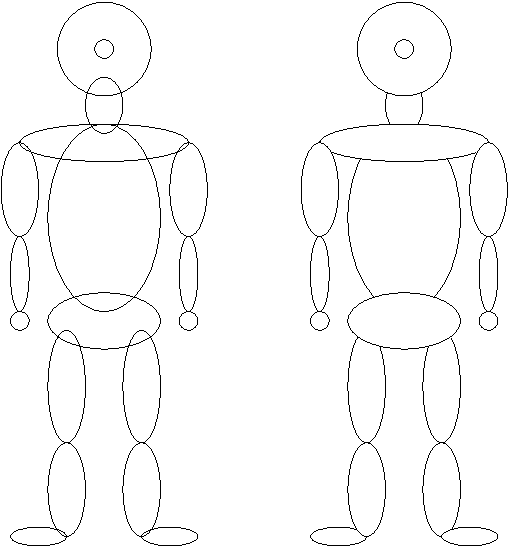
\psfig{file=blobby.eps,height=3in}\hfill~
\begin{center}
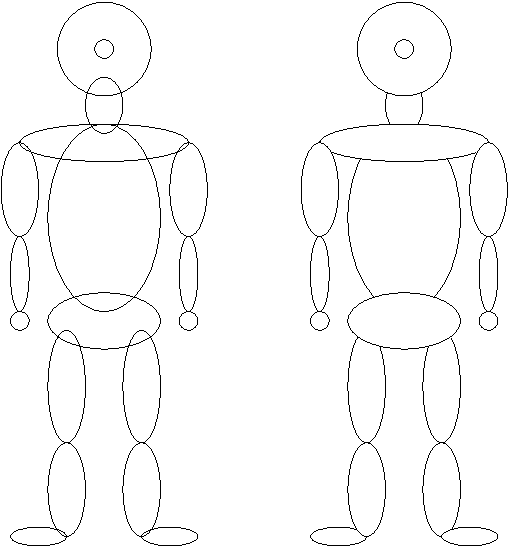
\includegraphics[height=3in]{blobby}
\end{center}

\noindent
where the figure on the left shows all overlapping, scaled spheres, and
the figure on the right has hidden surfaces removed (your puppet need
not have ``pigeon toes'').  The circle in the center of the face is a
nose.  You need at least one feature on the head so we can determine 
if rotations of the head are correct; it doesn't have to be a nose.  
Feel free to add eyes, ears, hair, mouth, antennae, etc., to your puppet.   

You can be creative with your model, as long as it has the same or more degrees
of freedom (number of joints) as this one.   In the past people
have built models of gorillas, dogs, Teddy bears, aliens, dinosaurs, 
gerbils, Oktoberfesters, etc.   
However, a ``creative'' model is not part of this assignment's
requirements.   Likewise you can add more modelling primitives
if you want beyond the sphere, but it's not a requirement. 

The coordinate system of each body part except the torso is 
therefore defined relative to a parent body part.
The dependencies are as shown:
\begin{center}
\begin{picture}(100,120)(-20,-120)
\put(0,0){Torso}
\put(-85,-20){\line(4,1){80}}
\put(110,-20){\line(-4,1){80}}
\put(-100,-30){Shoulders}
\put(-140,-50){\line(4,1){50}}
\put(-80,-37){\line(4,-1){50}}
\put(-175,-60){Left Upper Arm}
\put(-140,-67){\line(0,-1){15}}
\put(-170,-90){Left Forearm}
\put(-140,-97){\line(0,-1){15}}
\put(-165,-120){Left Hand}
\put(-85,-37){\line(0,-1){25}}
\put(-95,-75){Neck}
\put(-85,-82){\line(0,-1){15}}
\put(-95,-105){Head}
\put(-65,-60){Right Upper Arm}
\put(-30,-67){\line(0,-1){15}}
\put(-58,-90){Right Forearm}
\put(-30,-97){\line(0,-1){15}}
\put(-50,-120){Right Hand}

\put(115,-30){Hips}
\put(70,-50){\line(2,1){35}}
\put(175,-50){\line(-2,1){35}}
\put(70,-65){\line(0,-1){15}}
\put(50,-60){Left Thigh}
\put(70,-95){\line(0,-1){15}}
\put(52,-90){Left Calf}
\put(53,-120){Left Foot}
\put(175,-65){\line(0,-1){15}}
\put(150,-60){Right Thigh}
\put(175,-95){\line(0,-1){15}}
\put(152,-90){Right Calf}
\put(153,-120){Right Foot}
\end{picture}
\end{center}

The nose has been left out of this hierarchy as it is part of the Head
body part.

\bigskip
You are to implement primitives to build and render an
arbitrary hierarchical model.  You will then write a Lua script to
build a hierarchical data structure to represent the puppet.
Note the above structure is a physical representation of which
part of the body is connected to what, not the actual data structure.
For the actual data structure, you will need additional intermediate 
``transformation nodes'' for each body part to get the spheres properly 
hinged at the ends and for the joints.   It's also a good idea to not
put children under nodes with nonuniform scales; create childless
side branches instead.  In particular, you will only want to put
primitives at leaf nodes.

The definition of the puppet is to include {\bf fifteen} free angles,
three for each arm and leg, and three for the head and neck.
These angles will be used to animate the puppet.
The three arm angles will set the amount of rotation of the upper arm
forward about the shoulder, the amount of rotation of the forearm
forward about the elbow, and the amount of rotation of the hand backward 
and forward about the wrist, in the same plane as the elbow and shoulder.

The three leg angles will set the amount of rotation of the thigh
forward about the hip, the amount of rotation of the calf 
downward about the knee, and the amount of rotation of the foot
forward and backward about the ankle.

Of the remaining three angles,
one will set the amount of rotation of the base of the
neck forward with respect to the torso/shoulder, one 
will set the amount of rotation of the base of the head
forward with respect to the neck,
and the last will set the rotation of the head to the right or left
relative to the neck.

All angles will have minimum and maximum values which the interface
will enforce.   For example, it should not be possible to rotate
a knee or elbow the ``wrong way'', or to rotate a hand or foot more than
90 degrees from its neutral position.

{\bf Caution:} In the past, students have found the creation of
this model to be the most time consuming part of this assignment.
You will probably want to design it on paper before writing the
Lua code for the model.   

\section{Modelling}

You are to model your puppet using a Lua script.  The next section
describes the Lua/C++ interface you need to implement.  First, we 
take a quick look at how the interface is organized.

Lua is a simple scripting language. By using Lua to describe our scene
we do not have to write a special-purpose parser for the scene.
In C++, our scene will be represented as a number of
\texttt{Scene\-Node} instances. Each \texttt{Scene\-Node} object has a
transformation associated with it, and may have child nodes. There are
two classes derived from \texttt{Scene\-Node}: \texttt{Joint\-Node}
and \texttt{Geometry\-Node}. These classes represent special types of
nodes. Geometry nodes are nodes at which actual geometry is present
(in this assignment, spheres). Joint nodes are nodes which can be
manipulated in the user interface to rotate joints of the
puppet. 

To begin constructing a puppet, we need a root for our modelling hierarchy.
We can get one by asking for a transform node and assigning the result to
a Lua variable.  The name passed to the function is useful for debugging
purposes.
\begin{verbatim}
myroot = gr.node('root') 
\end{verbatim}
Functions like {\tt gr.sphere} create new geometry nodes.  We can then use
{\tt add\_child} to make a newly-created sphere a child of the root node:
\begin{verbatim}
torso = gr.sphere('torso') 
myroot:add_child(torso)
\end{verbatim}
You may wonder why we used a colon instead of a period in the last
line. In Lua, ``\texttt{:}'' is used to call member functions on
objects and ``\texttt{.}'' is used to call regular functions or class
functions.
We might then set the material properties of and transform the torso:
\begin{verbatim}
torso:set_material(gr.material(...))
torso:translate(1.0, 2.0, 3.0)
\end{verbatim}
Finally, we simply return the root node of the puppet:
\begin{verbatim}
return myroot
\end{verbatim}

Conceptually, the transformation at a node is applied to both its 
geometry and its children, and matrices deeper in the tree
are premultiplied by matrices higher in the tree.   This assumes
that column vectors are used to represent points.

The tree given in the previous section just relates the pieces of the
puppet.  The tree you create for your program will need to have
additional joint nodes, containing transformations and a joint
rotation range.  You will transform these ``joint'' nodes to animate
your puppet.  You may also need extra nodes to prevent child nodes
from being affected by transformations meant to modify only the
geometry of a parent node.  Watch out, in particular, for scales.  You
generally will not want these in the middle of a chain of
transformations.

\section{The Interface} 
The interface of your program should have at least a menu bar and a
viewing area.  The menu bar will have (at least) an {\tt Application}
menu, an {\tt Edit} menu, a {\tt Mode} menu and an {\tt Options} menu.
In addition, when the graphics display is resized the aspect ratio
should be properly maintained---the rendering of the puppet might
change size, but its proportions should not become distorted.

The Lua interface functions have been written for you, but they call
other functions which you will need to implement. Here is a list of
Lua functions that have been implemented (in \texttt{scene\_lua.cpp}):

\begin{itemize}
\item \texttt{gr.sphere(\textit{name})} ---
  Return a sphere with name \textit{name}.
  The sphere should be centered at the origin with
  radius 1.

\item \texttt{gr.node(\textit{name})} --- 
  Return a node \textit{name} that
  just contains a transformation matrix, which is 
  initialized to the identity matrix. 

\item \texttt{gr.joint(\textit{name}, \{\textit{xmin, xinit, xmax}\}, \{\textit{ymin, yinit, ymax}\})} --- 
  Create a joint node with minimum rotation angles \textit{xmin} and
  \textit{ymin}, maximum rotation angles \textit{xmax} and \textit{ymax} and
  initial rotation angles \textit{xinit} and \texttt{yinit} about the
  x and y axes.

\item \texttt{onode:add\_child(\textit{cnode})} --- 
  Add \textit{cnode} as a child of \textit{pnode}.

\item \texttt{gr.material(\{\textit{dr, dg, db}\}, \{\textit{sr, sg, sb}\}, \textit{p})} ---
  Return a material with diffuse reflection
  coefficients $dr$, $dg$, $db$, specular reflection
  coefficients $sr$, $sg$, $sb$, and Phong coefficient $p$.

\item \texttt{node:set\_material(\textit{mat})} --- 
  Give the node \textit{node} material \textit{mat}.  
  Node materials can be changed at any time.

\item \texttt{node:rotate(\textit{axis}, \textit{angle})} ---
  Rotate \textit{node} about \textit{axis} (\texttt{'x'}, \texttt{'y'}
  or \texttt{'z'}) by \textit{angle} (in degrees).
  
\item \texttt{node:translate(\textit{dx, dy, dz}} ---
  Translate \textit{node} by \textit{(dx, dy, dz)}.
  
\item \texttt{node:scale(\textit{sx, sy, sz})} ---
  Scale \textit{node} by \textit{(sx, sy, sz)}.
\end{itemize}

You can partially verify your implementation with \texttt{a3mark.lua}
and \texttt{a3mark.png}.  The TAs will use this script to test some of 
the functionality of your assignment.

Note that while the Lua-C++ interface for these commands is
completely implemented for you (in \texttt{scene\_lua.cpp}), you will
need to fill in the stubs in \texttt{scene.cpp}, and extend the scene
data structures appropriately.

\subsection{Application Menu}
The {\tt Application} menu should have the following items:
\begin{description}
	\item[{\tt Reset Position}]---Reset the origin of the puppet to its 
		initial position.  Keyboard shortcut  \texttt{I}.
	\item[{\tt Reset Orientation}]---Reset 
		the puppet to its initial orientation.
		Keyboard shortcut  \texttt{O}.
	\item[{\tt Reset Joints}]---Reset all joint angles, and clear the
		undo/redo stack.
		Keyboard shortcut  \texttt{N}.
	\item[{\tt Reset All}]---Reset the position, orientation, and 
	 	joint angles of the puppet, and clear the undo/redo
		stack.
		Keyboard shortcut~\texttt{A}.
	\item[{\tt Quit}]---Terminate the program.
		Keyboard shortcut~\texttt{Q}.
\end{description}

\subsection{Mode Menu}
The {\tt Mode} menu should have the following radiobutton selections:
\begin{description}
	\item[{\tt Position/Orientation}]---Translate and
		rotate the entire puppet.
		Keyboard shortcut  \texttt{P}.
	\item[{\tt Joints}]---Control joint angles.
		Keyboard shortcut  \texttt{J}.
\end{description}
Initially, the program should be in the {\tt Position/Orientation} 
mode.  

The behaviour of this interface is detailed in the following.
\begin{description}
\item[{\tt Position/Orientation}:]
    The code in \texttt{\CourseData/demo/trackball} illustrates the
    interface you should implement for translating and rotating the
    puppet. You can use the \texttt{trackball.c} code here as a basis
    for your implementation.

    The following details the behavior of each mouse button.
    If you have questions about how this interface works,
    test {\tt intdemo} and make your interface match it.
    \begin{itemize}
	\item Dragging the mouse with B1 depressed changes the {\it x}
	    and {\it y} translation of the puppet. 
	\item B2 depressed changes the {\it z} translation; moving the
	    mouse up on the screen should move the puppet away from
	    the viewer, while moving the mouse down on the screen 
	    should move the puppet closer.
	\item Use B3 to implement a virtual trackball 
	    direct-manipulation-3D-orientation interface.
	    The ``virtual sphere'' should be centered on the screen
	    and its diameter should be 50\% of the width or height
	    of the raster widget, whichever is smaller.

The skeleton
code will display a circle centred on the screen.  This
circle corresponds to the virtual sphere.  The radius of the 
circle will be a quarter of \texttt{min(screen width, screen
height)}.  

	\end{itemize}

	The translation should be done relative to the view frame.
The rotation should also be performed relative to the view frame, 
translated to the puppet's origin.
Since in this assignment the view frame is fixed, you can make this
easy by putting the camera in a simple canonical world-frame position.
Rotating the puppet about its own origin can be done with an appropriate
transform node above the torso.

\item[{\tt Joints}:]
	Clicking B1 is used as an event to signal picking.
	The cursor will be used with this signal to
	select a part of the puppet model.

	Selecting is regarded as a toggle operation.
	If an item is unselected, and it is picked,
        it will become selected.
	If the same item is picked again, it will
	become unselected.
        Selecting an item should cause a visible change in the rendering
        of that item (change the material).

        Only items that are directly under a movable joint 
        should be selectable.   When an item is selected, the 
        joint immediately above it in the hierarchy will be affected
        by the user interface.    If an item is not selectable,
        i.e. it is not immediately under a movable joint,
        picking it should do nothing.   In particular, there should
        be no visible change in unselectable objects when they are 
        picked.  

	\emph{Multiple simultaneous selections should be permitted}.

	For all selected items, the
	relative mouse {\it y} motion with B2 pressed
	will be mapped to the angles of the joint immediately
        above each selected object in the hierarchy.  
        In addition, the head will rotate to the left and right
        with B3 depressed, in response to relative {\it x} motion of the mouse.
        It should be possible to depress both B2 and B3 simultaneously and
        simultaneously nod and rotate the head.
        The head should only move if it is selected, for both B2 and B3 
        motions.
\end{description}

\subsection{Edit Menu}
The {\tt Edit} menu should have the following items:
\begin{description}
	\item[{\tt Undo}]---undo the previous transformation on the
		undo/redo stack.
		Keyboard shortcut  \texttt{U}.
	\item[{\tt Redo}]---redo the next transformation on the
		undo/redo stack.
		Keyboard shortcut  \texttt{R}.
\end{description}

You should maintain an undo/redo stack of transformations.  All 
joint transformations should be saved to the stack.  The paradigm
is that when you release a mouse button when in joint manipulation
mode, the current joint angles are stored on the undo/redo stack.
Initially, the stack contains the ``reset'' joint angles.  
If we think of the stack as extending upwards, you should maintain
a current position in the stack.  Selecting
undo from the edit menu will restore the joint angles to the entry
below the current one on the stack (and update the stack pointer
to point at that entry).  Selecting redo will update the joint angles
to the entry above the current one on the stack (and update the
stack pointer to point at that entry).

If several joint transformations are undone, and a new joint transformation
is initiated, all undo/redo entries above the current one should be
cleared.  If Reset All or Reset Joints are selected from the File Menu,
the undo/redo stack should be cleared.  You should provide reasonable
feedback to indicate that an attempt to undo or redo past the end
of the stack has been attempted (and not allow the action).


\subsection{Picking Menu}

The {\tt Picking} menu should be implemented if you are unable to get
selection with the mouse working properly (objective 3).  Create a 
checkbox menu item for each selectable part.  You will not get a mark 
for objective 3, but you will be able to implement and demonstrate 
joint movements.


\subsection{Options Menu}
The {\tt Options} menu should have the following checkbox item:
\begin{description}
	\item[{\tt Circle}]---draws the circle for the trackball if checked.
		Keyboard shortcut  \texttt{C}.
	\item[{\tt Z-buffer}]---draws the puppet with the OpenGL z-buffer
		if checked.
		Keyboard shortcut  \texttt{Z}.
	\item[{\tt Backface cull}]---draws the puppet with backfacing
		polygons removed.
		Keyboard shortcut  \texttt{B}.
	\item[{\tt Frontface cull}]---draws the puppet with frontfacing
		polygons removed.
		Keyboard shortcut  \texttt{F}.
\end{description}
All options should default to being ``off''.

\section{OpenGL}
Most of what you need to learn about OpenGL is in the programming
guide and man pages.  However, here are a few items that are
hard to find, and a few hints to make the assignment easier.
None of the following are requirements on your program; they're
just hints that students in past terms have found helpful.
\begin{itemize}
	\item Unit normals.  To get the lighting calculation
		correct, you must use unit normals.  Although
		it is trivial to specify unit normals for the
		faces of the sphere, when you scale the sphere,
		the normals will also be scaled, making them
		of non-unit length.  To avoid this problem,
		use the appropriate {\tt glEnable} command to tell OpenGL
		automatically scale all normals to unit length.
	\item Material properties.  You can set ambient, diffuse,
		and specular material properties.  For debugging
		purposes, it is probably easiest if you turn off
		the specular material properties (or rather, if
		you never turn them on).
	\item Lights.  For debugging purposes, it is easiest to
		have a single light source, placed at the eye.
		This will allow you to decide more easily if
		the shading of the puppet looks correct.
        \item 3D Picking. 3D picking would require you to pass an index for each
                object that you draw. In the Fragment Shader, You then create a
                texture and write the index to the pixel location on that
                texture. After the entire scene is drawn, you get the mouse
                position and get the index from the texture that was genereated
                with the indices. 
                For more information, go to this
                \href{http://www.opengl-tutorial.org/miscellaneous/clicking-on-objects/picking-with-an-opengl-hack/}{OpenGL tutorial}.
\end{itemize}

You are required to use a {\em Vertex Buffer Object} to render the sphere. A
Vertex Buffer Object is a way of storing all vertices, normals, and color as
they are calculated so that OpenGL can reuse them rather than have to
recalculate (and retransmit) them to OpenGL. 

Although you may use the {\tt gluSphere} command if you want, you may
want to generate the sphere yourself using sines and
cosines, and drawing the sphere as a set of rectangles.  For extra
performance improvements, draw your puppet as a sequence of {\em quad
strips} (this is not required, though).  Regardless, you should select
a resolution of the sphere that results in a good quality sphere while
still allowing for smooth motion.

\section{Donated Code}
In \texttt{\CourseData/data/A3} you will find
\begin{itemize}
\item {\tt AppWindow.cpp} -- The application window.
\item {\tt main.cpp} -- The program entry point.
\item {\tt material.cpp} -- Classes and functions for manipulating
  materials.
\item {\tt primitive.cpp} -- Classes and functions for manipulating
  geometric primitives such as spheres, etc.
\item {\tt scene.cpp} -- Classes and functions defining modelling
  hierarchies.  The layout of these classes should provide
  some ideas about how to organize your code.
\item {\tt scene\_lua.cpp} -- The Lua/C++ interface.
\item {\tt Viewer.cpp} -- The QGLWidget OpenGL viewer widget.
\item {\tt Makefile} -- Used to build the program.
\item {\tt a3mark.lua} -- A Lua script to test your implementation.
\item {\tt a3mark.png} -- An image showing what the screen output
  of {\tt a3mark.lua} should look like.
\item {\tt shader.vert} -- Simple Vertex Shader
\item {\tt shader.frag} -- Simple Fragment Shader
\end{itemize}
These files have been copied to your \texttt{handin/A3} directory.
You should also use {\tt trackball.c} which you can find
in {\tt \CourseData/demo/trackball}.

Note that the matrix multiplication routines are not needed for rendering,
only to set up the matrices in the nodes.

\section{Deliverables}
\begin{description}
\item[Executables:] \hfill
  The following two files are to be in your \texttt{A3/} directory:
	\begin{description}
        \item \texttt{puppeteer} - Your puppet viewer. This program
          should take a single argument specifying a Lua puppet file
          to load. If no arguments are given it should load
          \texttt{puppet.lua} from the current directory.
	\item \texttt{puppet.lua} - Your puppet.
	\end{description}
	The supporting source code should also be available in the
	{\tt src} directory.

    Don't forget \texttt{screenshot01.png}.

\item[Documentation:] \hfill
	\begin{itemize}
	\item Document changes you make to the data structure.
	\item Document the structure of the hierarchical model of your puppet.
	\end{itemize}
\end{description}

For this assignment, you are encouraged to make creative models.
The instructor and TAs may assign up to 1 bonus mark for interesting
puppets.

\newpage
\section{Objectives: \hfill Assignment 3}

\noindent{\large \bf Due: \AthreeDeadline.} \bigskip

\noindent{\large \bf Name: \hrulefill} \bigskip

\noindent{\large \bf UserID: \hrulefill} \bigskip

\noindent{\large \bf Student ID: \hrulefill} \bigskip

\begin{description}
\item[\_\_\_ 1:]
        {\tt a3mark.lua} runs and displays correctly.
\item[\_\_\_ 2:]
	The puppet's proportions are reasonable
	and the spheres are joined together in a logical fashion.
	The spheres are ``hinged'' to their neighbours
	at their ends---they do not rotate about their centres.
\item[\_\_\_ 3:]
	Picking works correctly and reliably.
\item[\_\_\_ 4:]
	Selection records are kept correctly so that
	any sequence of picks-to-select and picks-to-unselect
	works.   Multiple selections are supported.
	Selected portions of the puppet are clearly 
	indicated---e.g. selected parts change colour, or their edges 
	are highlighted.
\item[\_\_\_ 5:]
	The puppet can be globally rotated and translated for viewing purposes.
	The rotation user interface is a virtual trackball.
	A circle representing the virtual sphere can be turned on or off from
	the menu. It must be clearly visible when it is turned on.
	The puppet's configuration can be reset from the menu.
\item[\_\_\_ 6:]
        A well-designed hierarchical data structure is employed.
	Each sphere is drawn as an instance of a single display
	list sphere.
\item[\_\_\_ 7:]
	The joint movements are correct and the angles are restricted
	so that no grossly unnatural configurations are allowed.
	The puppet does not fly apart or distort during any sequences
	or combinations of actions.
\item[\_\_\_ 8:]
	Z-buffer, backfacing and frontfacing polygon hidden surface 
	removal are implemented and each can be toggled on and off.
\item[\_\_\_ 9:]
	The puppet is lit such that its 3D structure is clearly
	visible.  
\item[\_\_\_ 10:]
	An undo/redo stack is maintained.
\end{description}

\vspace*{.1in}
{\bf Declaration:}
\begin{quote}
        I have read the statements regarding cheating in the \CourseNumber
        course handouts.
        I affirm with my signature that I have worked out my own solution
        to this assignment, and the code I am handing in is my own.

\end{quote}

        {\bf Signature:}
\vspace*{.1in}


